\includepdf{Tasks/Probl-manif1}
\newpage
\section*{Решения}
\subsection*{Задача 1}
	\begin{figure}[!h]
		\begin{minipage}[h]{0.49\linewidth}
			\center\includegraphics[width=0.75\linewidth]{Pic2}
		\end{minipage}
		\begin{minipage}[h]{0.49\linewidth}
			\center\includegraphics[width=0.9\linewidth]{Pic3}
		\end{minipage}
	\end{figure}
	\vskip 0.1in
	Сопоставим каждому треугольнику точку $a$ на $\mathbb{S}$ и длины сторон $l_1, l_2 > 0$. Таким образом мы построили биекцию $\varphi: \triangle \to (a, l_1, l_2)$.
	\begin{gather*}
		a \in \mathbb{S},\ l_1, l_2 \in \mathbb{R}_{+} \rightarrow (a,l_1,l_2) \in \mathbb{S} \times \mathbb{R} \times \mathbb{R}
	\end{gather*}
	Открытые множества $U_1 \times U_2 \times U_3 \subset \mathbb{S} \times \mathbb{R} \times \mathbb{R}$.\\
	Карты на $S^{1} \times \mathbb{R}_{+} \times \mathbb{R}_{+}$ -- это $(U_1 \times U_2 \times U_3,\ \varphi_1 \times \varphi_2 \times \varphi_3)$
	\vskip 0.2in
	Карты на $S^{1}$ -- 2 интервала $S^{1} \slash A_1$ и $S^{1} \slash A_2$, эти каты согласованы. $\varphi_2 \circ \varphi_1^{-1}(a) = \varphi_2(b) = c$
	\vskip 0.1in
	Карты на $\mathbb{R}_{+}$ это $((a,b),f)$
	\begin{gather*}
		f = f_1 \circ f'_1\\
		f'_1:\ x \to -\frac{2}{a-b} x + \frac{a+b}{a-b} = \frac{a+b-2x}{a-b} \text{ то есть } (a,b) \to (1,1)\\
		f_1:\ x \to \tan \frac{\pi x}{2}
	\end{gather*}
	Тогда $(a,b) \sim \mathbb{R}$
	\vskip 0.1in
	Проверим согласованность карт $((a,b), f_{ab})$ и $((c,d), f_{cd})$
	\begin{gather*}
		(f_1 \circ f'_1)^{-1} = {f'_1}^{-1} \circ f_1^{-1}\\
		f_2 \circ (f'_2 \circ {f'_1}^{-1}) \circ f_1^{-1} = \frac{x(b-a) + (a+b) - (c+d)}{d-c}\\
		x \in (c,b)
	\end{gather*}
	\begin{gather*}
		y_1 = \frac{2x-(a+b)}{b-a}\\
		x = \frac{2y-(a+b)}{b-a}\\
		y_2 = \frac{x(b-a)+(a+b)}{2}\\
		y_1 \circ y_2 = x\\
		y_2 \circ y_1 = x
	\end{gather*}
	Следовательно отображение линейное, откуда следует что оно биективное и $c-1$ диффеоморфизм\\
	Таким образом все карты $(U_1 \times U_2 \times U_3,\ \varphi_1 \times \varphi_2 \times \varphi_3)$ согласованы.
\newpage
\subsection*{Задача 2}
\begin{enumerate}
	\item[(а)]$x^2+y^2+z^2=1$\\
		$A_1, A_2$ -- полюса
		Пусть $U_1 = S^2 \slash A_1,\ U_2 = S^2 \slash A_2$
		\begin{gather*}
			\varphi_1: (x,y,z) \to \left(\frac{x}{1-z}, \frac{y}{1-z}\right)\\
			\varphi_2: (x,y,z) \to \left(\frac{x}{1+z}, \frac{y}{1+z}\right)
		\end{gather*}
		\begin{figure}[!h]
			\includegraphics[width=0.7\linewidth]{Pic1}
		\end{figure}
		\vskip 0.2in
		Отображение перехода\\
		\begin{gather*}
			\varphi_{12} = \varphi_2 \circ \varphi_1^{-1}\\
			(x,y,z) \ne (0,0,\pm 1)\\
			\varphi_1^{-1}(x,y) = \left(\frac{2x}{|a|^2+1}, \frac{2y}{|a|^2+1}, \frac{|a|^2-1}{|a|^2+1}\right)\\
			|a|^2=x^2+y^2\\
			\varphi_{12} = \left(\frac{x}{|a|^2}, \frac{y}{|a|^2}\right) = \left(\frac{x}{x^2+y^2}, \frac{y}{x^2+y^2}\right)\\
			J = 
			\begin{vmatrix}
				\frac{y^2-x^2}{(x^2+y^2)^2} & \frac{-2xy}{(x^2+y^2)^2}\\
				\frac{-2xy}{(x^2+y^2)^2} & \frac{x^2-y^2}{(x^2+y^2)^2}
			\end{vmatrix}
			=
			\frac{1}{(x^2+y^2)^2}
			\begin{vmatrix}
				y^2-x^2 & -2xy\\
				-2xy & x^2-y^2
			\end{vmatrix}
			\ne 0
		\end{gather*}
		Следовательно отображение гладкое
	
	\item[(б)]
		зададим $A_1, A_2, U_1, U_2$ аналогично пункту (а)
		\begin{gather*}
			\varphi_1:\ (x_0, \ldots, x_n) = \left(\frac{x_0}{1-x_n},\ldots,\frac{x_{n-1}}{1-x_n}\right)\\
			\varphi_2:\ (x_0, \ldots, x_n) = \left(\frac{x_0}{1+x_n},\ldots,\frac{x_{n-1}}{1+x_n}\right)\\
			\varphi_2 \circ \varphi_1^{-1}:\ (x_0, \ldots, x_n) = \left(\frac{x_1}{x_1^2 + \ldots + x_n^2},\ldots,\frac{x_{n}}{x_1^2 + \ldots + x_n^2}\right)
		\end{gather*}
		Следовательно оно гладкое\\
		Посчитаем Якобиан
		\begin{gather*}
			\frac{\partial \varphi_{12}}{\partial x_1} = \frac{x_1^2 + \ldots + x_n^2 - 2x_1^2}{(x_1^2 + \ldots + x_n^2)^2} = \frac{-x_1^2 + \ldots + x_n^2}{(x_1^2 + \ldots + x_n^2)^2}\\
			\frac{\partial \varphi_{12}}{\partial x_2} = \frac{-2x_1x_2}{(x_1^2 + \ldots + x_n^2)^2}\\
			\frac{1}{(x_1^2 + \ldots + x_n^2)^2} \cdot
			\begin{vmatrix}
				-x_1^2 + \ldots + x_n^2 & -2x_1x_2 & -2x_1x_3 & \ldots & -2x_1x_n\\
				-2x_1x_2 & x_1^2 - x_2^2 + \ldots + x_n^2 & \ddots & \ddots & \vdots\\
				-2x_1x_3 & \ddots & \ddots & \ddots & \vdots\\
				\vdots & \ddots & \ddots & \ddots & -2x_{n-1}x_n\\
				-2x_1x_n & \ldots & \ldots & -2x_{n-1}x_n & x_1^2 + \ldots + x_n^2
			\end{vmatrix}\\
			= 
			-(x_1^{2n} + \ldots + x_n^{2n}) + \ldots \ne 0
		\end{gather*}
	\item[(в)]
		Допустим что можно покрыть одной картой, тогда по определению карты существует гомеоморфизм $\varphi: \mathbb{S}^n \to \mathbb{R}^n$, но $S^n$ компакт, так как оно закрыто и ограничено (можно рассмотреть норму $|\ |: \mathbb{R}^n \to \left[0,+\infty \right)$ и $S^{n} = |\ |^{-1}(1)$), в то время как $\mathbb{R}^n$ не компакт так как его открытое покрытие $\{B(0, n)\ |\ n = 1, \ldots, \infty\}$ не имеет конечного подпокрытия.
\end{enumerate}


\subsection*{Задача 3}
	Заметим, что можно построить сюръективное отображение из множества ненулевых векторов(с началом в любой точке плоскости) во множество прямых на плоскости. Рассмотрим $A = \mathbb{R}^2 \times (\mathbb{R}^2 \slash 0)$, где перва точка отождествляется с началом вектора, а вторая является самим ненулевым вектором и введем на данном пространстве стандартную топологию. Теперь зададим отношение эквивалентности векторов $(p_1,v_1) \sim (p_2,v_2) \Leftrightarrow v_1 \parallel v_2 \wedge (p_1-p_2) \parallel v_1$. Таким образом мы можем отождествить $A  \slash \sim$ со множеством всех прямых плоскости и задать на нем стандартную фактор-топологию.\\
	Заметим, что любую прямую на плоскости можно задать как $ax + by + c =0$, таким образом построив биекцию с тройками $(a,b,c)$, причем можно заметить, что $(a,b,c) \sim (\lambda a, \lambda b, \lambda c)$ и тогда каждая прямая отождествляется с соответствующей ей тройкой в однородных координатах $ax + by + c \to (a:b:c)$ и множество прямых является подмножеством $RP^2$ (так как там отсутствует точка $a=b=0$).\\
	
	%можно сказать что эту выколотую точку можно растянуть в диск, а лента мебиуса с диском является проективной плоскостью
	\begin{figure}[!h]
		\includegraphics[width=0.9\linewidth]{Pic4}
	\end{figure}

\newpage
\subsection*{Задача 4}
\begin{enumerate}
	\item[(а*)]
	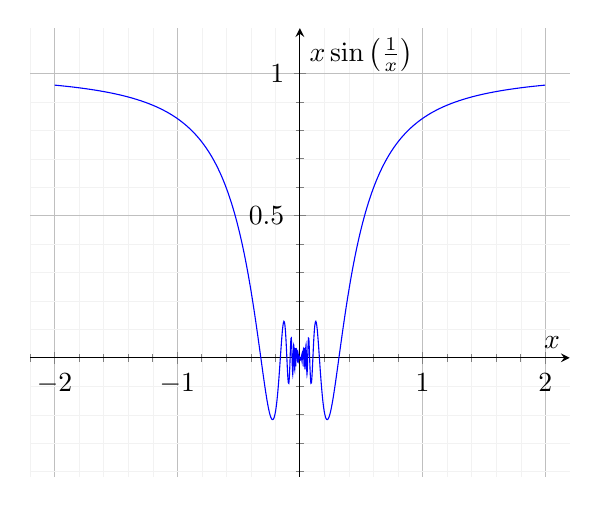
\begin{tikzpicture}
		\begin{axis}[
			grid=both,
			minor tick num=4,
			grid style={line width=.1pt, draw=gray!10},
			major grid style={line width=.2pt,draw=gray!50},
			axis lines=middle,
			enlargelimits={abs=0.2},
			xlabel=$x$,
			ylabel={$x \sin \left( \frac{1}{x}\right)$}
			] 
			\addplot[domain=-2:2,samples=1000,smooth,blue]{x*(sin(deg(1/x)))};
		\end{axis}
	\end{tikzpicture}
	\begin{gather*}
		\lim\limits_{x \to 0} x \sin \left(\frac{1}{x}\right) = 0
	\end{gather*}
	$|\sin \left(\frac{1}{x}\right)|<1$ ограничена, а $x=0$ при $x \to 0$ следовательно функция непрерывна в 0\\
	Если функция гладкая то её производная существует и непрерывна
	\begin{gather*}
		f' = \sin \frac{1}{x} + x \cos \frac{1}{x} \cdot -\frac{1}{x^2} = \sin \frac{1}{x} - \frac{1}{x} \cos \frac{1}{x}
	\end{gather*}
	$\sin \frac{1}{x}$ имеет разрыв в 0, а следовательно и $f'$ имеет разрыв, откуда следует что $f$ не гладкая.
	
	\item[(б)]
	\myuline{Гладкая кривая} -- это гладкое отображение $f: I \to \mathbb{R}^n$, где $I \subset \mathbb{R}$ является открытым множеством. Геометрическим объектом в данном случае является $f(I) \subset \mathbb{R}$\\
	\myuline{Регулярная кривая} -- это гладкая кривая $f: I \to \mathbb{R}^n$ для которой выполнено что $\forall t \in I:\ \dot{f}(t) \ne 0$\\
	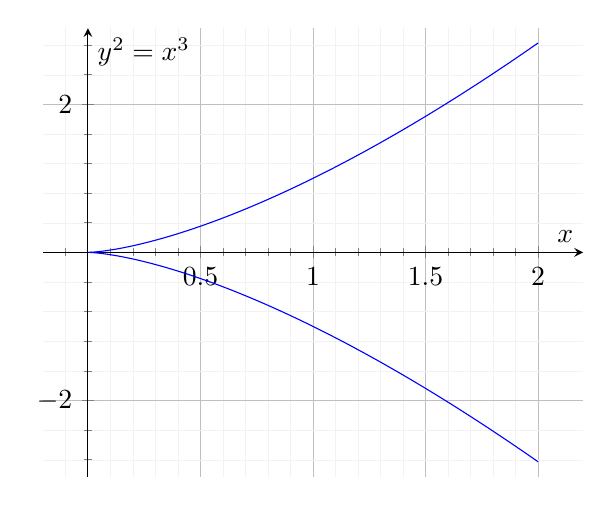
\begin{tikzpicture}
		\begin{axis}[
			grid=both,
			minor tick num=4,
			grid style={line width=.1pt, draw=gray!10},
			major grid style={line width=.2pt,draw=gray!50},
			axis lines=middle,
			enlargelimits={abs=0.2},
			xlabel=$x$,
			ylabel={$y^2 = x^3$}
			] 
			\addplot[domain=-2:2,samples=1000,smooth,blue]{sqrt{x^3}};
			\addplot[domain=-2:2,samples=1000,smooth,blue]{-sqrt{x^3}};
		\end{axis}
	\end{tikzpicture}
	\begin{gather*}
		\gamma:(-\infty, \infty) \to \mathbb{R}^{2}\\
		t \to (t^2, t^3)\\
		\frac{\partial t^2}{\partial t} \ne 0\\
		\frac{\partial t^3}{\partial t} \ne 0
	\end{gather*}
	Дифференцируема, а следовательно гладкая
	\begin{gather*}
		||v|| = ||(2t,3t^2)|| = \sqrt{4t^2 + 9t^2} = 0 \text{ при } t=0
	\end{gather*}
\end{enumerate}

\newpage
\subsection*{Задача 5}
	Пусть $(x_0^1, \ldots, x_0^n)$ -- координаты точки $x_0$ в пространстве $\mathbb{R}^n$ и $\frac{\partial f}{\partial x^i}(x_0) \ne 0$. Рассмотрим точку $v_0 = (x_0^1, \ldots, x_0^{i-1}, x_0^{i+1}, \ldots, x_0^{n}) \in \mathbb{R}^{n-1}$. Согласно теореме о неявной функции существует окрестность $v_0 \in V_i \subset \mathbb{R}^{n-1}$, интервал $(x_0^{i} - \delta, x_0^{i} + \delta)$ и гладкая функция $y^{i}: V_{i} \to \mathbb{R}$ такие что:
	\begin{gather*}
		x_0^{i} = y^i (x_0^{1}, \ldots, x_0^{i-1}, x_0^{i+1}, \ldots, x_0^{n})\\
		|x_0^{i} - y^i(x^1, \ldots, x^{i-1}, x^{i+1}, \ldots, x^n)| < \delta \text{ на } V_i\\
		\text{множество } U_i = \delta_c \cap (V \times (x_0^{i} - \delta, x_0^{i} + \delta)) \subset \mathbb{R}^n \text{ совпадает с множеством }\\ \{(x^{1}, \ldots, x^{i-1}, y^i(x^1, \ldots, x^{i-1}, x^{i+1}, \ldots, x^{n}), x^{i+1}, \ldots, x^{n})\ |\ (x^{1}, \ldots, x^{i-1}, x^{i+1}, \ldots, x^{n}) \subset V\}
	\end{gather*}
	Рассмотрим $(U_i, \varphi_i)$ в качестве карты в окрестности точки $x_0$.\\
	Это возможно так как $\varphi_i(U_i) = V_i$ и обратное отображение задается равенством $\varphi_i^{-1}(x^{1}, \ldots, x^{i-1}, x^{i+1}, \ldots, x^{n}) = (x^{1}, \ldots, x^{i-1}, y^i(x^{1}, \ldots, x^{i-1}, x^{i+1}, \ldots, x^{n}), x^{i+1}, \ldots, x^{n})$\\
	Отображение перехода $\varphi_j \varphi_i^{-1}:\ \varphi(U_i \cap U_j) \to V_j$ имеет вид $(x^{1}, \ldots, x^{i-1}, x^{i+1}, \ldots, x^{n}) \to ({x'}^{1}, \ldots, {x'}^{j-1}, {x'}^{j+1}, \ldots, {x'}^{n})$ где $x^{a} = x'^{a}$ при $a \ne i$ и ${x'}^{i} = y^{i}(x^{1}, \ldots, x^{i-1}, x^{i+1}, \ldots, x^{n})$ и, следовательно, гладкое.


\subsection*{Задача 6}
	Поверхность $f(x_1, \ldots, x_n) = 0$\\
	\myuline{Карты регулярной поверхности} -- локальные окрестности $x \in U$, которым гомеоморфно $V \subset \mathbb{R}^{n}$ (некое открытое множество)\\
	Тогда каждое множество, удовлетворяющее условию, будет картой, рассмотрим 2 из них\\
	Проверим согласованность карт $(U_1, f_1),\ (U_2, f_2)$ в точке $x = (x_1, \ldots, x_n)$
	\begin{gather*}
		f_1(x_1, \ldots, x_n) = f(x_2, x_3, \ldots, x_n)\\
		f_2(x_1, \ldots, x_n) = f(x_1, x_3, \ldots, x_n)\\
		f_{12} = f_2 \circ f_1^{-1}(x_2, x_3, \ldots, x_n) = f_2(f_1(x_2, \ldots, x_n), x_2, \ldots, x_n) = (f_1(x_2, \ldots, x_n), x_3, \ldots, x_n)\\
		x_1 = f_1(x_2, \ldots, x_n)\\
		x_2 \to f_1(x_2, \ldots, x_n)\\
		x_3 \to x_3\\
		\ldots\\
		x_n \to x_n\\
		J = 
		\begin{vmatrix}
			\frac{\partial f_1}{\partial x_1} & \frac{\partial f_1}{\partial x_3} & \ldots & \frac{\partial f_1}{\partial x_n}\\
			0 & 1 & 0 & 0\\
			0 & 0 & 1 & 0\\
			0 & 0 & 0 & 1
		\end{vmatrix}
		\ne 0
		\text{ так как } \frac{\partial f_1}{\partial x_1} \ne 0 \text{ так как теорема о неявной функции применима}
	\end{gather*}

\newpage
\subsection*{Задача 7}
\begin{enumerate}
	\item[(а)]
		$(\mathbb{R}, \varphi), (\mathbb{R}, \psi)$ -- гладкие структуры\\
		\begin{gather*}
			\varphi(x) = x^{2k+1}\\
			\psi(x) = x^{2n+1}\\
			k \ne n
		\end{gather*}
		Атласы $(\mathbb{R}, \varphi)$ и $(\mathbb{R}, \psi)$ не одинаковые, так как $\bigcup$ атласов не является атласом.
		\begin{gather*}
			\psi \circ \varphi^{-1}(x) = x^{\frac{2n+1}{2k+1}}\\
			\varphi \circ \psi^{-1}(x) = x^{\frac{2k+1}{2n+1}}\\
			x^{\frac{2n+1}{2k+1}} \cdot x^{\frac{2k+1}{2n+1}} = x\\
			\text{следовательно } J \left(x^{\frac{2n+1}{2k+1}}'\right) = J \left(\frac{2n+1}{2k+1} \cdot x^{\frac{2k+1}{2n+1}-1}\right) \text{ или } J \left(x^{\frac{2k+1}{2n+1}}'\right) = J \left(\frac{2k+1}{2n+1} \cdot x^{\frac{2n+1}{2k+1}-1}\right)\\
			\text{ не существует в точке } x=0
		\end{gather*}
		Следовательно карты не согласованы и отображение перехода не гладкое
		\begin{gather*}
			\exists f: \varphi(x) \to \psi(x)\\
			f: x \to x^{\frac{2k+1}{2n+1}}
		\end{gather*}
		\begin{figure}[!h]
			\includegraphics[width=0.5\linewidth]{Pic5}
		\end{figure}\\
		Тогда $g: x \overset{id}{\to} \psi \circ f \circ \varphi^{-1}(x) = x$ -- диффеоморфизм
	\item[(б)]
	\item[(в*)]
\end{enumerate}

\subsection*{Задача 8*}
